\documentclass[]{exam}

%These tell TeX which packages to use.
\usepackage{array,epsfig}
\usepackage{amsmath}
\usepackage{amsfonts}
\usepackage{amssymb}
\usepackage{amsxtra}
\usepackage{amsthm}
\usepackage{mathrsfs}
\usepackage{color}
\usepackage{array}
\usepackage{graphicx}
\graphicspath{ {../art/} }
\usepackage{bm}
\usepackage{tikz}
\usepackage{multicol}
\usepackage{enumitem}

\renewcommand\qedsymbol{$\blacksquare$}

%Here I define some theorem styles and shortcut commands for symbols I use often
\theoremstyle{definition}
\newtheorem{defn}{Definition}
\newtheorem{thm}{Theorem}
\newtheorem{cor}{Corollary}
\newtheorem*{rmk}{Remark}
\newtheorem{lem}{Lemma}
\newtheorem*{joke}{Joke}
\newtheorem{ex}{Example}
\newtheorem*{soln}{Solution}
\newtheorem{prop}{Proposition}

\newcommand{\lra}{\longrightarrow}
\newcommand{\ra}{\rightarrow}
\newcommand{\surj}{\twoheadrightarrow}
\newcommand{\graph}{\mathrm{graph}}
\newcommand{\bb}[1]{\mathbb{#1}}
\newcommand{\Ell}{\mathscr{L}}
\newcommand{\Z}{\bb{Z}}
\newcommand{\Q}{\bb{Q}}
\newcommand{\R}{\bb{R}}
\newcommand{\C}{\bb{C}}
\newcommand{\N}{\bb{N}}
\newcommand{\M}{\mathbf{M}}
\newcommand{\m}{\mathbf{m}}
\newcommand{\MM}{\mathscr{M}}
\newcommand{\HH}{\mathscr{H}}
\newcommand{\Om}{\Omega}
\newcommand{\Ho}{\in\HH(\Om)}
\newcommand{\bd}{\partial}
\newcommand{\del}{\partial}
\newcommand{\bardel}{\overline\partial}
\newcommand{\textdf}[1]{\textbf{\textsf{#1}}\index{#1}}
\newcommand{\img}{\mathrm{img}}
\newcommand{\ip}[2]{\left\langle{#1},{#2}\right\rangle}
\newcommand{\inter}[1]{\mathrm{int}{#1}}
\newcommand{\exter}[1]{\mathrm{ext}{#1}}
\newcommand{\cl}[1]{\mathrm{cl}{#1}}
\newcommand{\ds}{\displaystyle}
\newcommand{\vol}{\mathrm{vol}}
\newcommand{\cnt}{\mathrm{ct}}
\newcommand{\osc}{\mathrm{osc}}
\newcommand{\LL}{\mathbf{L}}
\newcommand{\UU}{\mathbf{U}}
\newcommand{\support}{\mathrm{support}}
\newcommand{\AND}{\;\wedge\;}
\newcommand{\OR}{\;\vee\;}
\newcommand{\Oset}{\varnothing}
\newcommand{\st}{\ni}
\newcommand{\wh}{\widehat}

%Pagination stuff.
\setlength{\topmargin}{-.3 in}
\setlength{\oddsidemargin}{0in}
\setlength{\evensidemargin}{0in}
\setlength{\textheight}{9.in}
\setlength{\textwidth}{6.5in}

\newcommand{\id}[1]{\mbox{\it #1\/}}
\newcommand{\rid}[1]{\mbox{\rm #1}}
\newcommand{\sid}[1]{\mbox{\sf #1}}
\newcommand{\bid}[1]{\mbox{\bf #1}}
\newcommand{\tinysz}[1]{\mbox{\tiny $#1$}}



\newcommand{\twonode}{%
  \begingroup\normalfont
  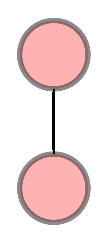
\includegraphics[height=\fontcharht\font`\b]{2nodetree.eps}%
  \endgroup
}


\title{Lab 4: Proving Properties of Mutually Recursive Systems}
\author{Foundations of Computer Science}
\date{\today}
%\pagestyle{empty} 
%\footer{}{\thepage}{}

\begin{document}

\maketitle

\setlength{\columnseprule}{1pt}
\section*{Post System Practice}
\begin{questions}
\question Write a Post system that defines the negative integers.
\question Write a Post system that defines even natural numbers greater than $6$.
\question Consider the following Post systems:
\begin{multicols}{2}
\begin{tabbing}
{\bf R2}XX \=  \kill
{\bf B} \>
        \(\begin{array}[t]{l}
        a \in S
        \end{array}\) \\[2ex]
{\bf R} \>
        \(\begin{array}[t]{l}
        x \in S \;\;\;y \in S \\
        \hline
        xy \in S
        \end{array}\)
\end{tabbing}

\begin{tabbing}
{\bf R2}XX \=  \kill
{\bf B} \>
        \(\begin{array}[t]{l}
        a \in T
        \end{array}\) \\[2ex]
{\bf R} \>
        \(\begin{array}[t]{l}
        x \in T \\
        \hline
        xx \in T
        \end{array}\)
\end{tabbing}

\end{multicols}
\begin{parts}
\part Write definitions for $S$ and $T$ using set comprehension notation.
\part Is $S$ equal to $T$?
\part Bonus practice: Prove $T \subseteq S$.
\end{parts}

\question Consider the following Post system:

\begin{tabbing}
{\bf R2}XX \=  \kill
{\bf B} \>
        \(\begin{array}[t]{l}
        1 \in N
        \end{array}\) \\[2ex]
{\bf R1} \>
        \(\begin{array}[t]{l}
        x \in N \\
        \hline
        x\times x \in S
        \end{array}\)\\[2ex]
{\bf R2} \>
        \(\begin{array}[t]{l}
        x \in S \;\;\; y \in N \\
        \hline
        x+y \in N
        \end{array}\)
\end{tabbing}
\begin{parts}
\part List $5$ elements of $S$ and $5$ elements of $N$.
\part Use set comprehension notation to write definitions of $S$ and $N$. 
\end{parts}


\uplevel{\section*{Trees}
Answer the questions below referring to the following definitions:
\begin{itemize}
\item A ``leaf'' node is a node with no children.
\item An ``internal'' node is a node that is not a leaf.
\item A full binary tree is a tree in which every internal node
      has exactly two children.
\item An extended binary tree is a tree in which every internal
      node has one or two children.
\end{itemize}}
\hrule
%This week: strong induction vs. weak induction.
%Mutual recursive definition and mutual induction.

\question Write a Post System for full binary trees.

\question Write a Post System for extended binary trees.

\question Let $L$ be the number of leaf nodes and $I$ be the number
          of internal nodes. Suppose you are asked to prove that for all 
          full binary trees, $L = I + 1$.
\begin{parts}
\part What induction rule should you use? 
\part What variable will you perform induction over? 
\part Set up the proof: write the base case, inductive hypothesis and inductive step.
\part Prove the base case.
\part Prove the inductive step.
\end{parts}
\uplevel{\section*{Simple Automata}}
\question The diagram below shows a slightly modified version of the simple
switch discussed in class. \\
\begin{figure}[h]
\centering
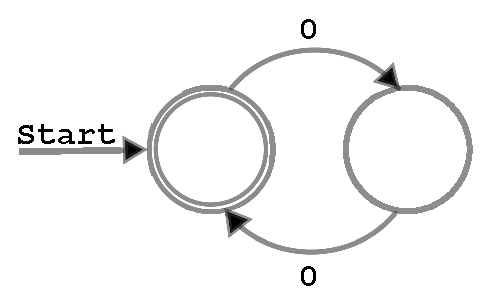
\includegraphics[width=2.5in, height=.75in,keepaspectratio=true]{evenzeroautomata.eps}
\label{2sp}
\end{figure}

There are two changes:
\begin{itemize}
\item Instead of a button labeled ``Push,'' this machine has a single button
labeled ``0''. Pressing the button represents sending the character ``0''
to the machine, which results in a state transition, just as it did when labeled
``Push'' in the previous version.
\item The double circle shown for the start state indicates that this is an
``accepting'' state. If the machine is in an accepting state after processing
all its input, it has accepted the input. If it ends in any other state, it has
rejected the input.
\end{itemize}
For the following questions, let $L$ be the set of all strings accepted by this machine. 
We refer to this set as the language recognized by the machine.

\begin{parts}
\part What is the alphabet of $L$?
\part Define $L$ using set comprehension notation. 
\part What induction rule would you use to prove that all the strings contained
in the set $L$ as you have defined it are accepted by the machine? What variable 
should you do induction over?
\part What induction rule would you use to prove that all the strings accepted 
by the machine are contained in the set $L$ as you have defined it? What
variable should you do induction over?
\part Which of the above proves soundness of the machine with respect to $L$, and 
which proves completeness? 
\part Sketch the proof of completeness.
\part Prove the base case. 
\part Prove the inductive step.
\end{parts}

\end{questions}
\end{document}


